% Untangling Federal Jurisdiction
% Part 2 of 3

% All content comes from Stephen Pratt. I have no idea if he approves of this effort or not.

\documentclass{beamer}
\usetheme{Madrid}
%\usetheme{Goettingen}
\usefonttheme{serif}
\usefonttheme{structuresmallcapsserif}
% \usepackage[font=small,labelfont=bf]{caption}
\usepackage{xcolor}
\usepackage{rotating}

\setbeamerfont{section title}{parent=title}
\setbeamercolor{section title}{parent=titlelike}
\defbeamertemplate*{section page}{default}[1][]
{
    \centering
    \begin{beamercolorbox}[sep=8pt,center,#1]{section title}
        \usebeamerfont{section title}\insertsection\par
    \end{beamercolorbox}
}
\newcommand*{\sectionpage}{\usebeamertemplate*{section page}}

\def\Put(#1,#2)#3{\leavevmode\makebox(0,0){\put(#1,#2){#3}}}

\makeatletter
\setbeamertemplate{footline}
{
    % Commented out to remove footer line entirely
%    \leavevmode%
%    \hbox{%
%    \begin{beamercolorbox}[wd=.333333\paperwidth,ht=2.25ex,dp=1ex,center]{author in head/foot}%
%        \usebeamerfont{author in head/foot}\insertshortauthor%~~\beamer@ifempty{\insertshortinstitute}{}{(\insertshortinstitute)}
%    \end{beamercolorbox}%
%    \begin{beamercolorbox}[wd=.333333\paperwidth,ht=2.25ex,dp=1ex,center]{title in head/foot}%
%        \usebeamerfont{title in head/foot}\insertshorttitle
%    \end{beamercolorbox}%
%    \begin{beamercolorbox}[wd=.333333\paperwidth,ht=2.25ex,dp=1ex,right]{date in head/foot}%
%        \usebeamerfont{date in head/foot}\insertshortdate{}\hspace*{2em}
%        \insertframenumber{} / \inserttotalframenumber\hspace*{2ex} 
%    \end{beamercolorbox}}%
%    \vskip0pt%
}
\makeatother

\newenvironment<>{varblock}[2][\textwidth]{
    \begin{center}
        \begin{minipage}{#1}
            \setlength{\textwidth}{#1}
            \begin{actionenv}#3
                \def\insertblocktitle{#2}
                \par
                \usebeamertemplate{block begin}}
            {\par
                \usebeamertemplate{block end}
            \end{actionenv}
        \end{minipage}
    \end{center}
}

\DeclareGraphicsExtensions{.pdf,.png,.jpg}


\begin{document}
\unitlength=1pt

\section{Clause Family Martyred}
\frame{\sectionpage}

\begin{frame}{South Carolina v. United States, 1905}
    \centering
    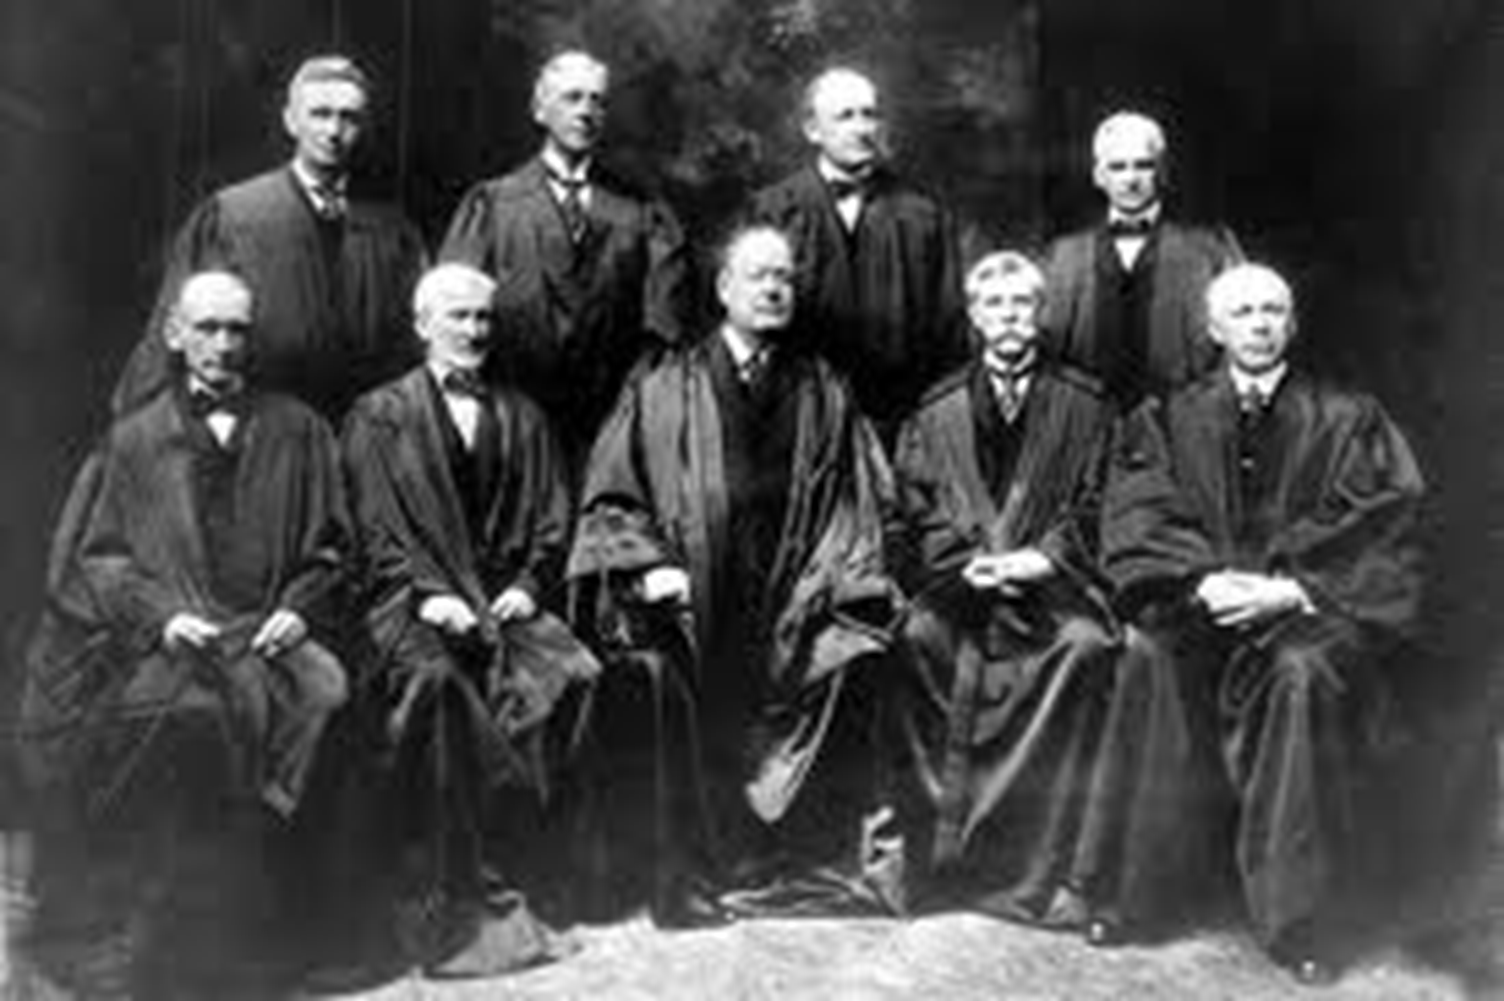
\includegraphics[width=0.75\textwidth]{img/sc-1905.png} \\
    ``The Constitution is a written instrument. As such, its meaning does not alter. That which it meant when it was adopted, it means now.'' \\
\end{frame}

\begin{frame}{United States v. Sprague, 1931}
    \centering
    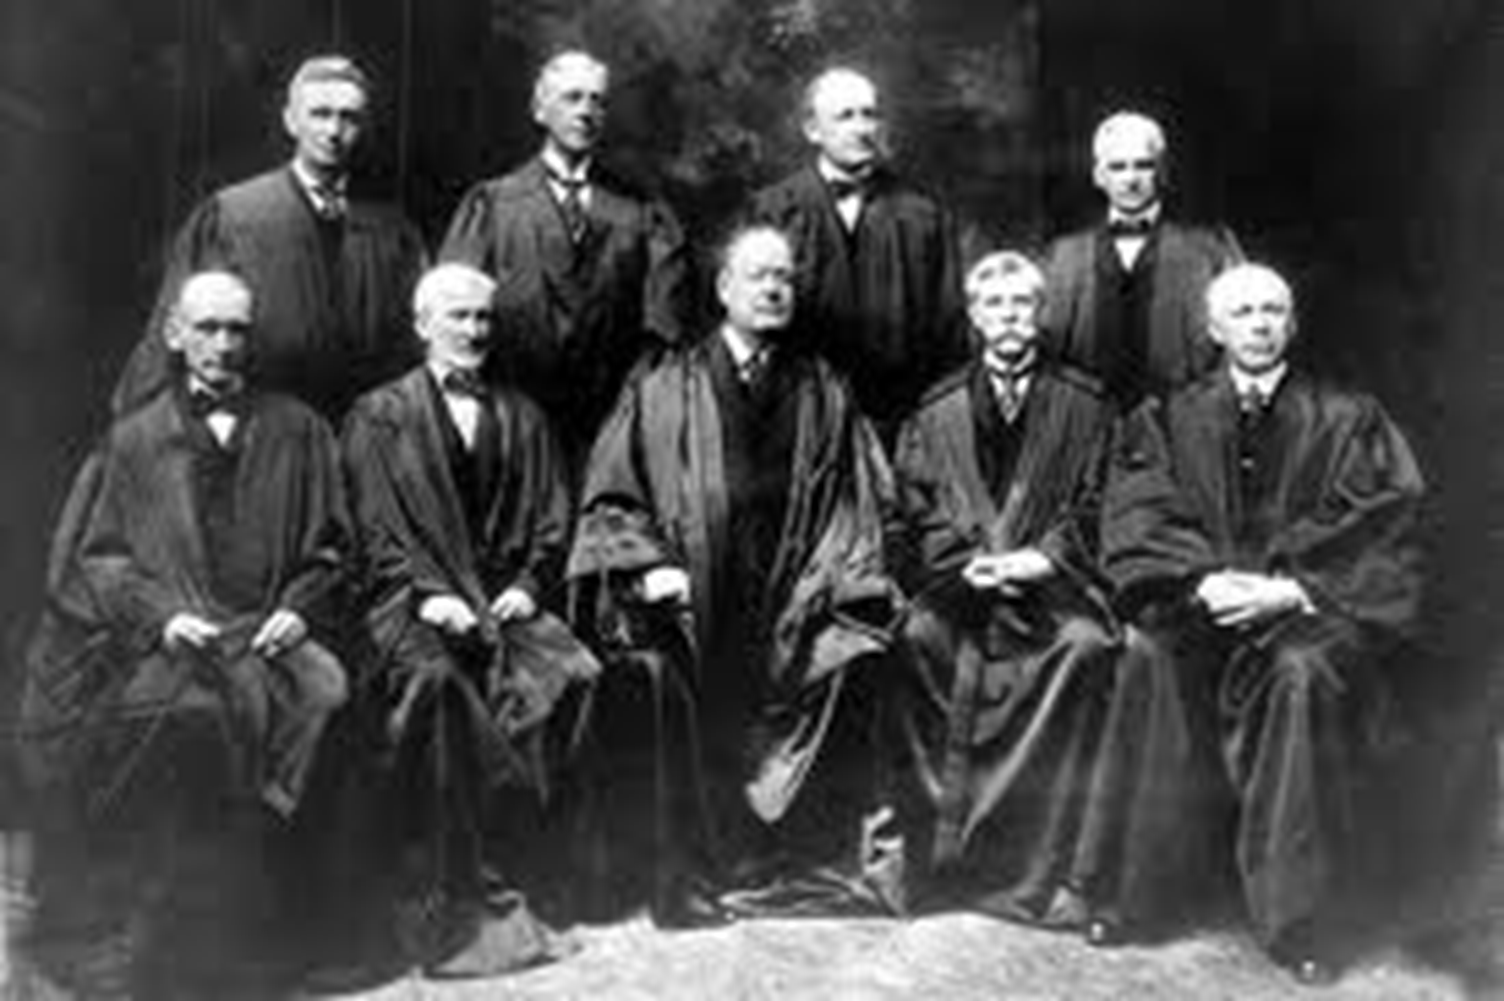
\includegraphics[width=0.75\textwidth]{img/sc-1905.png} \\
    ``The Constitution was written to be understood by the voters; its words and their phrases were used in their normal and ordinary\ldots meaning.'' \\
\end{frame}

\begin{frame}
    \begin{columns}[c]
        \column{0.5\textwidth}
            \centering
            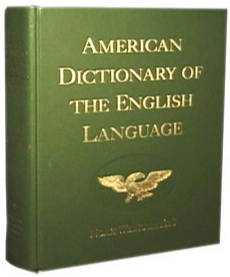
\includegraphics[width=0.75\textwidth]{img/dictionary.png} \\
        \column{0.5\textwidth}
            \centering
            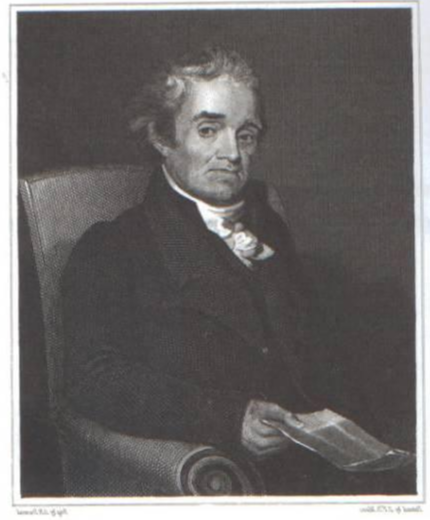
\includegraphics[height=0.5\textheight]{img/noah-webster.jpg} \\
            \only<1>{Published by Noah Webster in 1828 \\}
            \only<2>{\textbf{Engagement:} Obligation by agreement or contract. \\}
    \end{columns}
\end{frame}

\begin{frame}{Jurisdiction Clause Family --- Engagement}
    \centering
    
\includegraphics[height=0.85\textheight]{img/family.png} \\
    \huge{\textbf{ \color{white}
        %\Put(25, 300){\begin{sideways}\colorbox{blue}{Admissions}\end{sideways}}
        %\Put(60, 300){\begin{sideways}\colorbox{blue}{Claims}\end{sideways}}
        %\Put(90, 300){\begin{sideways}\colorbox{blue}{Property}\end{sideways}}
        %\Put(134, 300){\begin{sideways}\colorbox{blue}{Guarantee}\end{sideways}}
        %\Put(168, 300){\begin{sideways}\colorbox{blue}{Enclave}\end{sideways}}
        \Put(200, 300){\begin{sideways}\colorbox{blue}{Engagements}\end{sideways}}
        %\Put(235, 300){\begin{sideways}\colorbox{blue}{Supremacy}\end{sideways}}
    }}
\end{frame}

\begin{frame}{Engagement Clause}
   \centering
   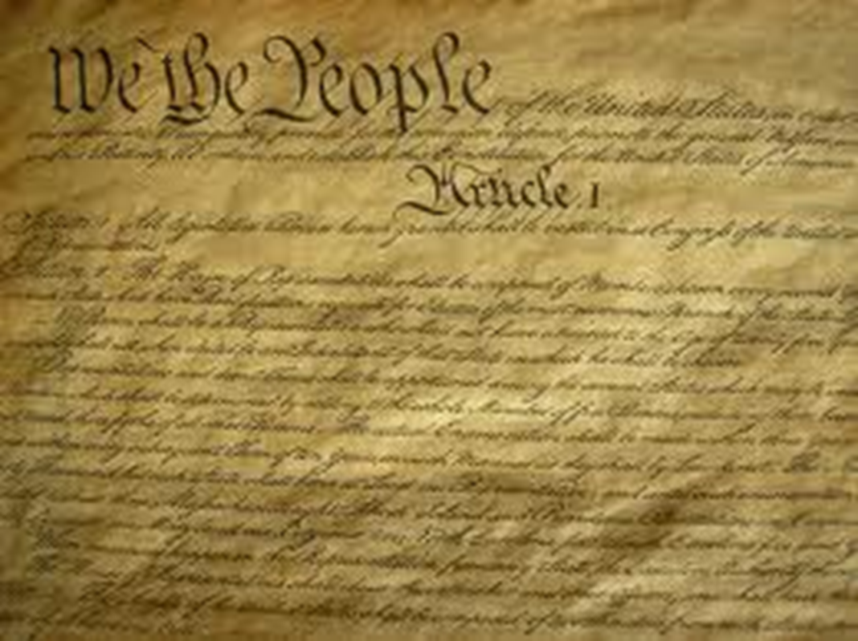
\includegraphics[height=.7\textheight]{img/constitution.png} \\
   \textbf{Article VI, clause 1:} ``\emph{Engagements} entered into, \emph{before} the Adoption of this Constitution, shall be as valid against the United States under this Constitution, as under the Confederation.''
\end{frame}

\begin{frame}{Articles of Confederation, on Federal Property}
    \begin{columns}[c]
        \column{0.5\textwidth}
            \centering
            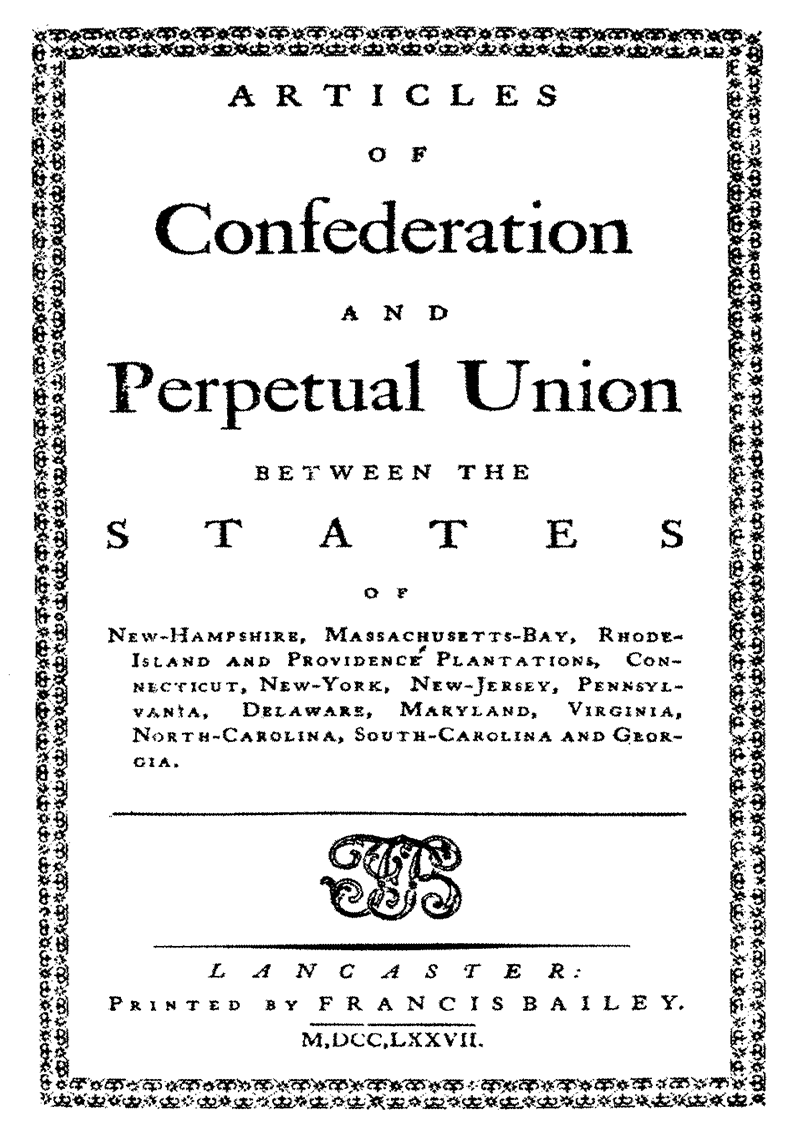
\includegraphics[width=0.75\textwidth]{img/articles-of-confederation.png} \\
        \column{0.5\textwidth}
            \textbf{Article IX:} \\
            ``\ldots no State shall be deprived of territory for the benefit of the United States.''
    \end{columns}
\end{frame}

\begin{frame}
    \begin{block}{}
        Formation of a ``more perfect union'' does not absolve that union of prior engagements, including those obligations established by the Resolution of 1780 and the Articles of Confederation.''
    \end{block}
\end{frame}

\begin{frame}{Johnson v. McIntosh, 1823}
    \centering
    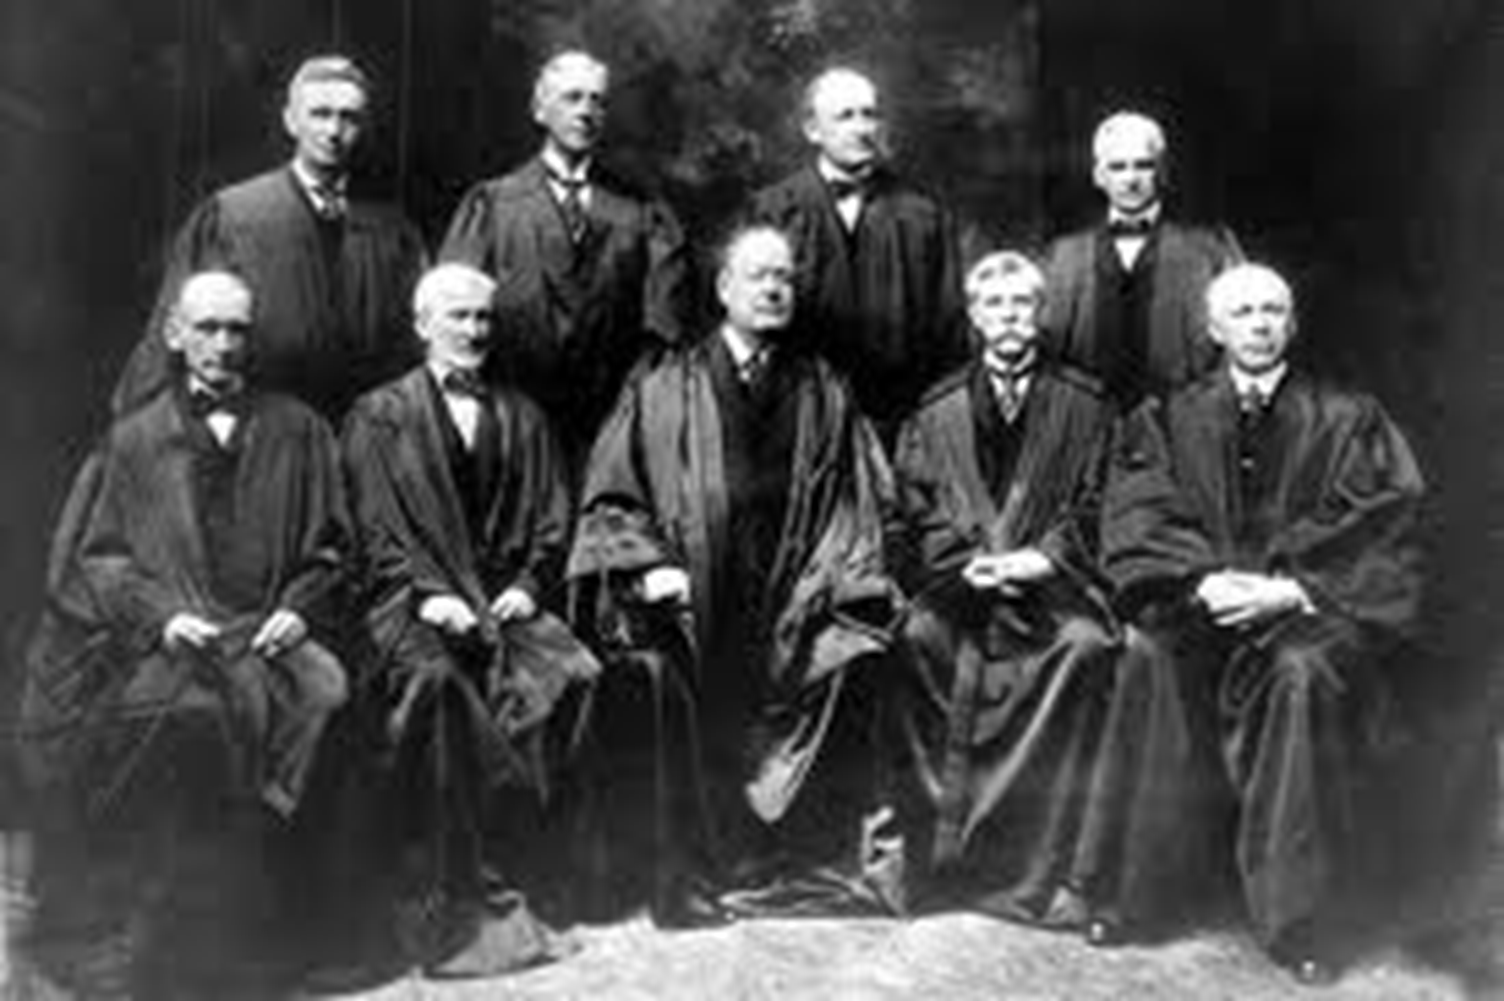
\includegraphics[width=0.75\textwidth]{img/sc-1905.png} \\
    ``And the \emph{vacant soil is to be disposed of} by that organ of the government which has the constitutional power to dispose of the national domain.'' \\
\end{frame}

\begin{frame}{Friedman v. Goodwin, 1856}
    \centering
    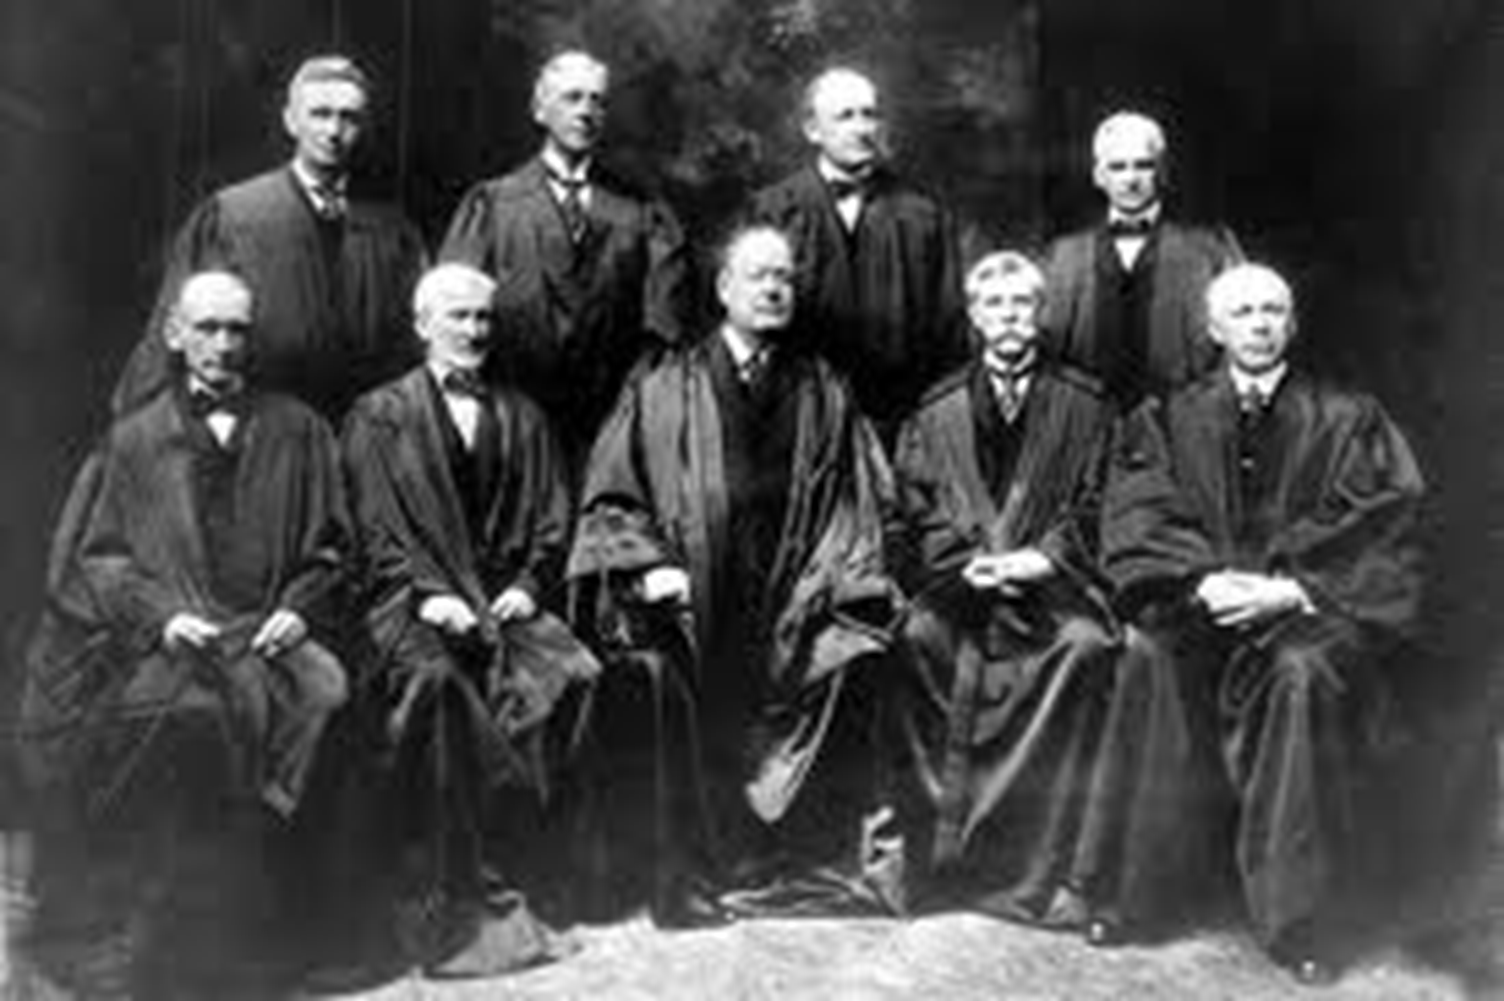
\includegraphics[width=0.75\textwidth]{img/sc-1905.png} \\
    ``On [California's] admission into the Union, \emph{she became the owner of all the public land} not disposed of by law of congress.'' \\
\end{frame}

\begin{frame}{Sovereign States, 1788}
    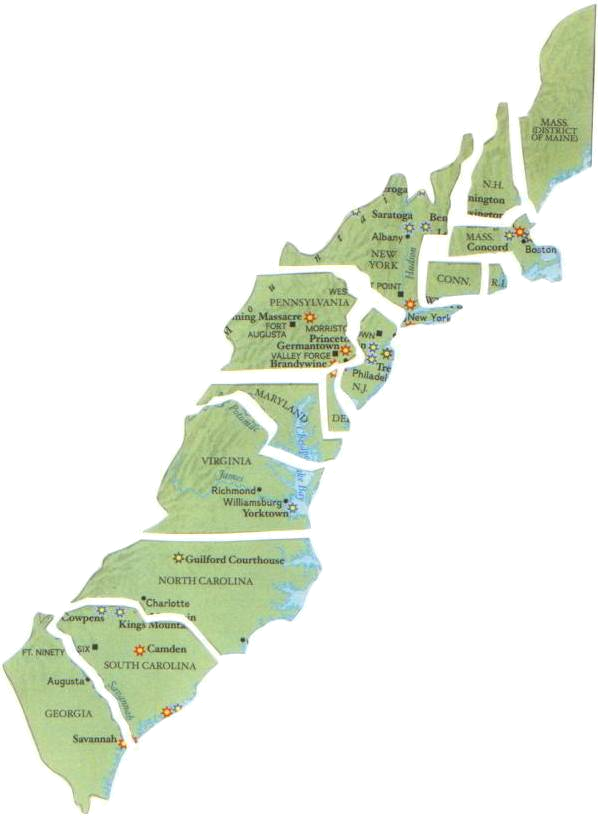
\includegraphics[height=0.75\textheight]{img/colonies.png} \\
    \pause
    \Put(200,300){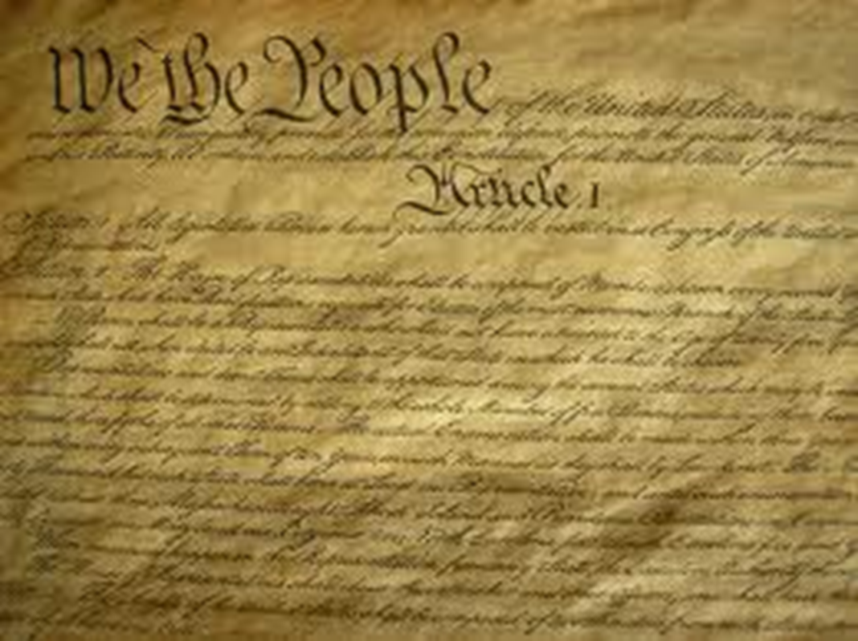
\includegraphics[width=0.4\textwidth]{img/constitution.png}}
    \Put(195,420){\textbf{List of delegated powers}}
    \pause
    \Put(200,60){
\includegraphics[width=0.3\textwidth]{img/national-seal.png}}
    \Put(225,170){\textbf{\Large{Agent}}}
\end{frame}

\begin{frame}{James Madison, 1821}
    \begin{columns}[c]
        \column{0.5\textwidth}
            \centering
            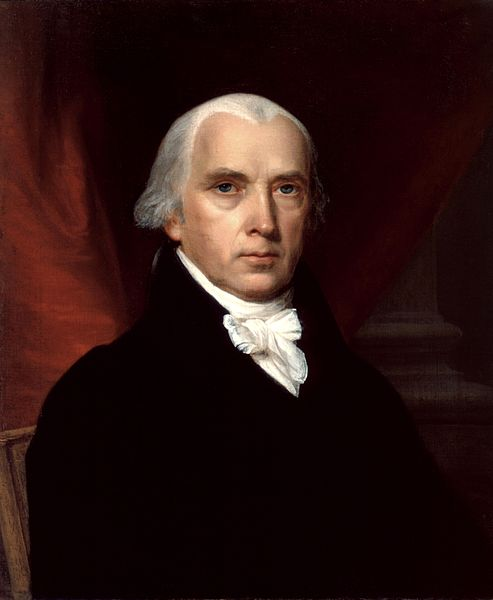
\includegraphics[width=0.75\textwidth]{img/madison.jpg} \\
        \column{0.5\textwidth}
            ``Our government system is established by \emph{compact}, not between the Government of the United States and the State Governments, but between the \textbf{states as sovereign communities}.''
    \end{columns}
\end{frame}

\begin{frame}{Two Contending Forces}
    \begin{columns}[c]
        \column{0.5\textwidth}
            \centering
            \large{Hamiltonian} \\
            \vspace{15pt}
            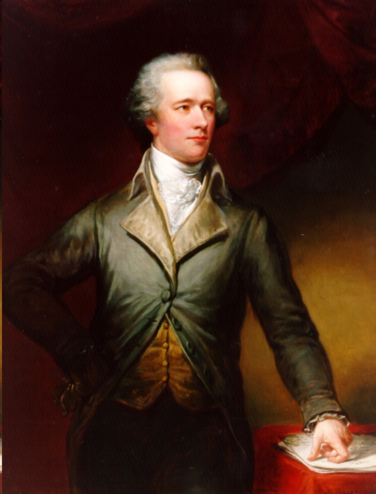
\includegraphics[height=0.60\textheight]{img/hamilton-portrait.png} \\
        \column{0.5\textheight}
            \centering
            \large{Jeffersonian} \\
            \vspace{15pt}
            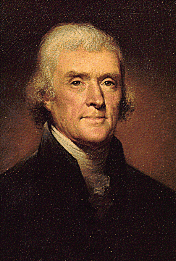
\includegraphics[height=0.60\textheight]{img/jefferson.png} \\
    \end{columns}
    \pause
    \vspace{20pt}
    On the 4th of July, we praise Jefferson, but we live in Hamilton's world.
\end{frame}

\begin{frame}
    \begin{columns}[c]
        \column{0.5\textwidth}
            \centering
            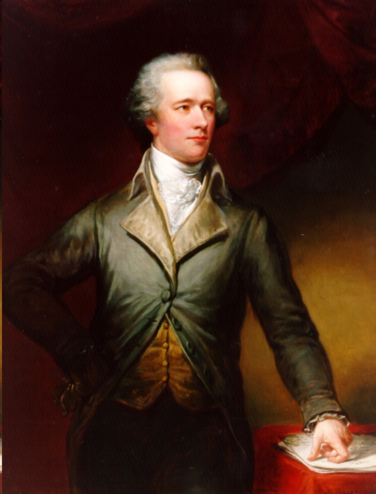
\includegraphics[height=0.60\textheight]{img/hamilton-portrait.png} \\
            Alexander Hamilton \\
        \column{0.5\textheight}
            ``The greatest man who ever lived was Julius Caesar."
    \end{columns}
\end{frame}

\begin{frame}{Two Contending Forces}
    \begin{columns}[c]
        \column{0.5\textwidth}
            \centering
            \large{Hamiltonian} \\
            \vspace{15pt}
            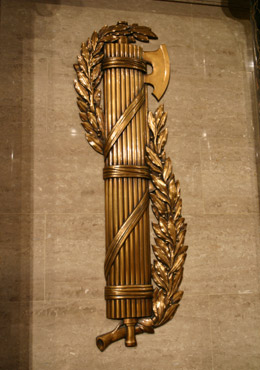
\includegraphics[height=0.60\textheight]{img/fasces.png} \\
        \column{0.5\textheight}
            \centering
            \large{Jeffersonian} \\
            \vspace{15pt}
            \pause
            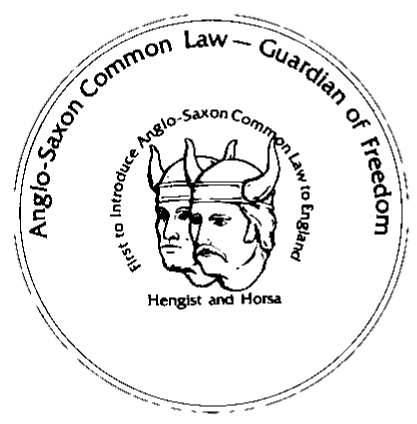
\includegraphics[height=0.60\textheight]{img/hh-coin.png} \\
    \end{columns}
\end{frame}

\begin{frame}{Summary}
    Sovereignty is possession of the highest power. It is impossible for both
    the states and the federal government to possess the highest power at the
    same time. When the sovereign states created the Constitution, they
    delegated a few enumerated powers to their new agent called the Federal
    Government. \\
    \vspace{20pt}
    \pause
    { \color{red}\textbf{\emph}They did not ``surrender many of their powers to the Federal Government''}
\end{frame}

\begin{frame}{George Bancroft}
    \begin{columns}[c]
        \column{0.5\textwidth}
            \centering
            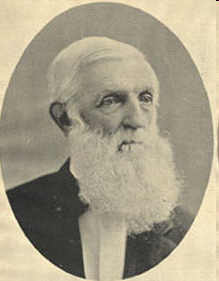
\includegraphics[width=0.75\textwidth]{img/george-bancroft.png} \\
            George Bancroft, 1800 - 1891 \\
        \column{0.5\textheight}
            \centering
            \textbf{A PLEA FOR THE CONSTITUTION OF THE UNITED STATES} \\
            Wounded in the house of its guardians \\
            \vspace{30pt} 1886, 25 pages \\
    \end{columns}
\end{frame}

\begin{frame}{George Bancroft}
    \begin{columns}[c]
        \column{0.5\textwidth}
            \centering
            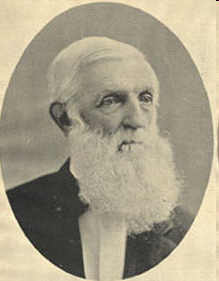
\includegraphics[width=0.75\textwidth]{img/george-bancroft.png} \\
            George Bancroft, 1800 - 1891 \\
        \column{0.5\textheight}
            ``The government of the United States is far, very far removed from the powers of a sovereign state.''
    \end{columns}
\end{frame}

\begin{frame}{Sovereignty}
\begin{table}[h]
\centering
\begin{tabular}{p{.48\textwidth} p{.48\textwidth}} 
    { \centering \huge{Consolidationists} \\ } & { \centering \huge{State's rights} \\ } \\
    { \centering 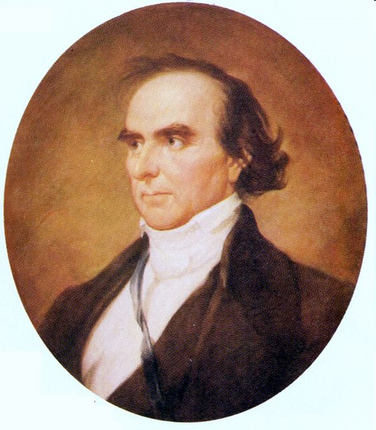
\includegraphics[height=0.45\textheight]{img/daniel-webster-portrait.png} \\ } &
        { \centering 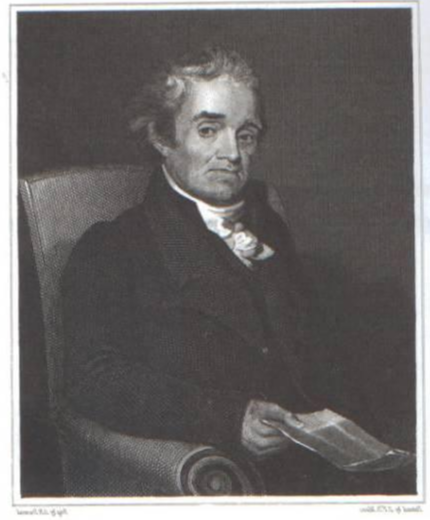
\includegraphics[height=0.45\textheight]{img/noah-webster.jpg} \\ } \\
    \only<1>{{\centering Daniel Webster \\ } & {\centering Noah Webster \\ } \\ }
    \only<2>{ { \centering \textbf{Sovereignty:} The sum of all rights and powers \\ } &
      { \centering \textbf{Sovereignty:} Supreme in power; \ldots the highest power \\ } \\ }
\end{tabular}
\end{table}
\end{frame}

\begin{frame}{``Consolidating School''}
    \begin{columns}[c]
        \column{0.5\textwidth}
            \centering
            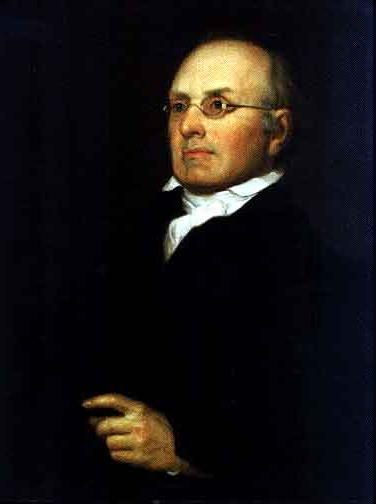
\includegraphics[height=0.4\textheight]{img/story-portrait.png} \\
            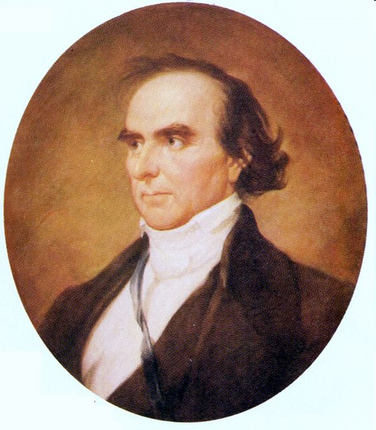
\includegraphics[height=0.4\textheight]{img/daniel-webster-portrait.png} \\
        \column{0.5\textheight}
            Sovereignty is the sum of all rights and powers. \\
            In the Constitution sovereignty is delegated to the central government, which is an irrevocable \emph{ceding} of power.
    \end{columns}
\end{frame}

\begin{frame}{``Consolidating School''}
    \begin{columns}[c]
        \column{0.5\textwidth}
            \centering
            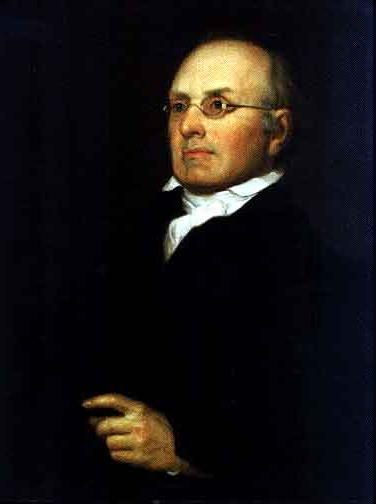
\includegraphics[height=0.4\textheight]{img/story-portrait.png} \\
            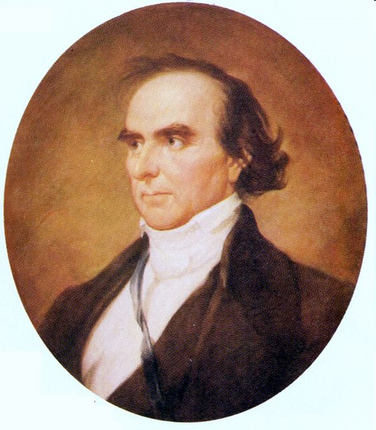
\includegraphics[height=0.4\textheight]{img/daniel-webster-portrait.png} \\
        \column{0.5\textheight}
            States have sovereignty, except so far as they have ceded it. \\
            \pause
            \vspace{30pt} \textbf{Dual Sovereignty}
    \end{columns}
\end{frame}

\begin{frame}{John Taylor of Caroline, 1823}
    \begin{columns}[c]
        \column{0.5\textwidth}
            \centering
            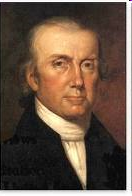
\includegraphics[height=0.4\textheight]{img/john-taylor-of-caroline.png} \\
        \column{0.5\textheight}
            The \emph{consolidating school} contends that we have two
            sovereignties; but that one is sovereign over the other; Mr.
            Hamilton, that we have co-ordinate sovereignties, but that one is
            made superlative.
    \end{columns}
\end{frame}

\begin{frame}{United States v. Gardner, 1997}
    \begin{columns}[c]
        \column{0.5\textwidth}
            \centering
            
\includegraphics[height=0.4\textheight]{img/federal-court.png} \\
        \column{0.5\textheight}
            ``The state government and the federal government exercise \emph{concurrent jurisdiction} over the land.''
    \end{columns}
\end{frame}

\begin{frame}{Concurrent Jurisdiction Defined}
    \begin{columns}[c]
        \column{0.5\textwidth}
            \centering
            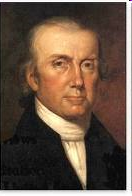
\includegraphics[height=0.4\textheight]{img/john-taylor-of-caroline.png} \\
        \column{0.5\textheight}
            \textbf{Concurrent Jurisdiction:} \\
            The \emph{consolidating school} contends that we have two
            sovereignties; but that one is sovereign over the other; Mr.
            Hamilton, that we have co-ordinate sovereignties, but that one is
            made superlative.
    \end{columns}
\end{frame}

\begin{frame}{Hamilton, 1788 newspaper}
    \begin{columns}[c]
        \column{0.5\textwidth}
            \centering
            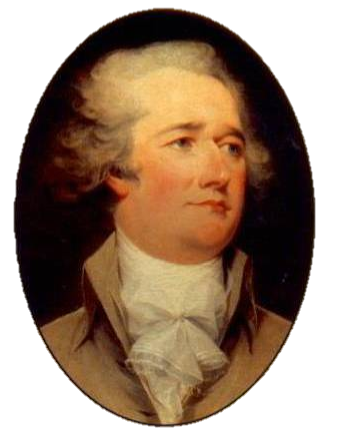
\includegraphics[width=0.75\textwidth]{img/hamilton.png} \\
        \column{0.5\textheight}
            \only<1>{``Imperium in imperio is a political monster''}
            \only<2>{``[A sovereign within a sovereign] is a political monster''}
    \end{columns}
\end{frame}

\begin{frame}{Kleppe v. New Mexico, 1976}
    \begin{columns}[c]
        \column{0.5\textwidth}
            \centering
            
\includegraphics[width=0.75\textwidth]{img/octopus.png} \\
            Department of the Interior \\
        \column{0.5\textheight}
            I have ``complete'' legislative power ``without limitation'' over Federal Lands!
    \end{columns}
\end{frame}

\begin{frame}{FLPMA, 1976}
    \begin{columns}[c]
        \column{0.5\textwidth}
            \centering
            
\includegraphics[width=0.75\textwidth]{img/octopus.png} \\
            Department of the Interior \\
        \column{0.5\textheight}
            \emph{At \textbf{my} discretion} I will offer contracts to state
            and local law enforcement officials to enforce Federal laws and
            regulations on public lands.
    \end{columns}
\end{frame}

\begin{frame}{Feds}
    \begin{columns}[c]
        \column{0.5\textwidth}
            \centering
            
\includegraphics[width=0.75\textwidth]{img/fed-fish.png} \\
        \column{0.5\textheight}
            You states don't forget the ``Supremacy Clause''! We are more sovereign than you are!
    \end{columns}
\end{frame}

\begin{frame}{Delegated powers, few and defined}
    \begin{columns}[c]
        \column{0.5\textwidth}
            \centering
            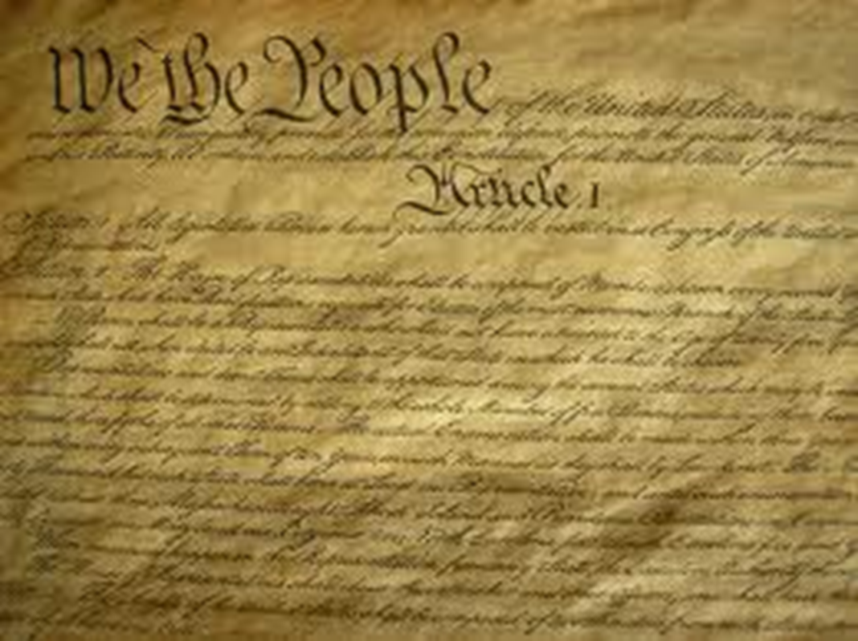
\includegraphics[width=0.75\textwidth]{img/constitution.png} \\
        \column{0.5\textheight}
            \begin{itemize}
                \item Coin money
                \item Declare war
                \item Raise armies
                \item Punish piracies
                \item etc.
            \end{itemize}
    \end{columns}
\end{frame}

\begin{frame}
    \begin{varblock}[0.8\textwidth]{Warning}
        Federal Public Servants: Your powers are few and defined. If it is not on the list, you CANNOT do it!
    \end{varblock}
\end{frame}

\begin{frame}
    Delegated powers are NOT sovereignty! They are simply the powers the
    sovereign states delegated (loaned) to their agent, the Federal Government.
\end{frame}

\begin{frame}
    \begin{columns}[c]
        \column{0.5\textwidth}
            \centering
            
\includegraphics[width=0.75\textwidth]{img/owl.png} \\
        \column{0.5\textheight}
            \Large{Do not confuse sovereignty with the powers which the sovereign delegates.}
    \end{columns}
\end{frame}

\begin{frame}{REMEMBER!}
    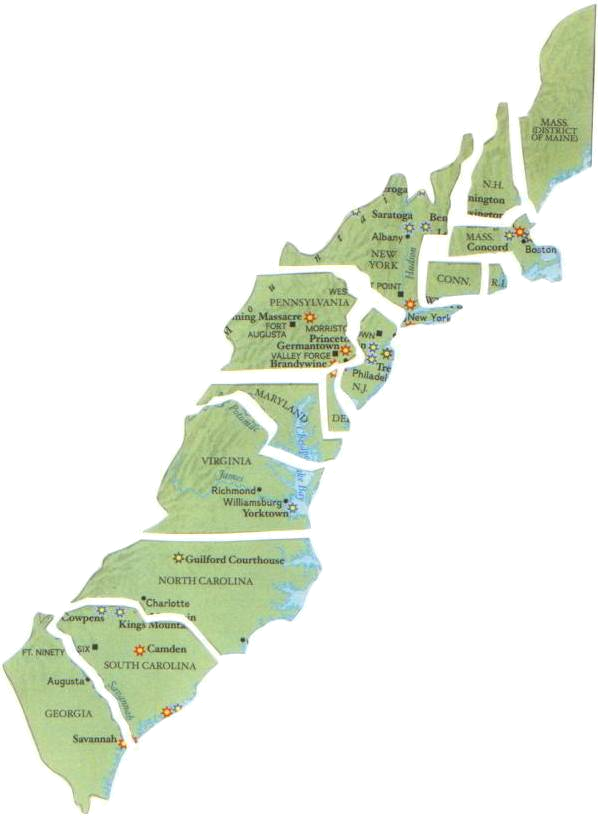
\includegraphics[height=0.75\textheight]{img/colonies.png} \\
    \Put(200,300){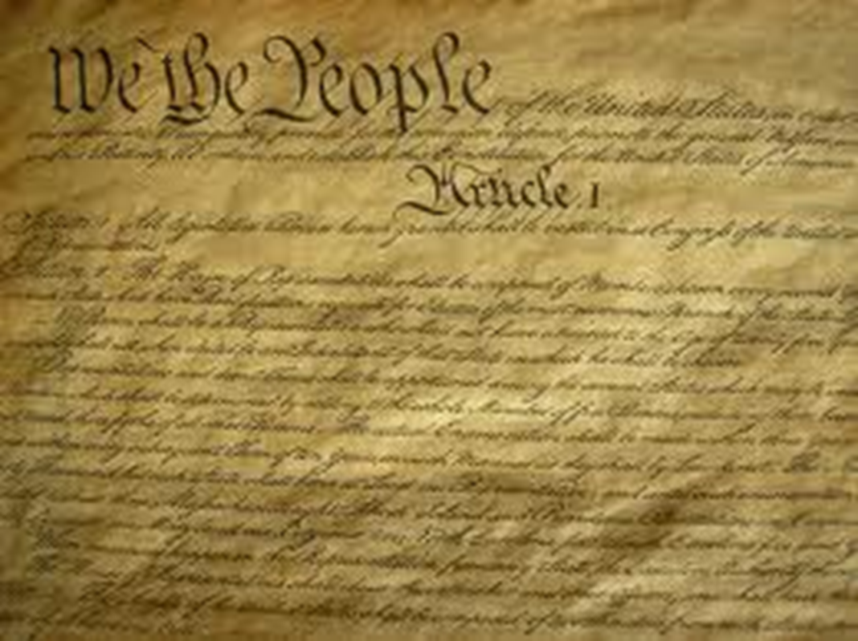
\includegraphics[width=0.4\textwidth]{img/constitution.png}}
    \Put(195,420){\textbf{List of delegated powers}}
    \Put(200,60){
\includegraphics[width=0.3\textwidth]{img/national-seal.png}}
    \Put(225,170){\textbf{\Large{Agent}}}
\end{frame}

\begin{frame}
    \begin{columns}[c]
        \column{0.5\textwidth}
            \Large{What if the agent does something that is not on the list?}
        \column{0.5\textheight}
            \centering
            
\includegraphics[width=0.95\textwidth]{img/kid-question.png} \\
    \end{columns}
\end{frame}

\begin{frame}{Resolutions of 1798}
    \begin{columns}[c]
        \column{0.5\textwidth}
            \Large{Each state is duty bound to ``interpose'' between the people and the federal government.}
        \column{0.5\textheight}
            \centering
            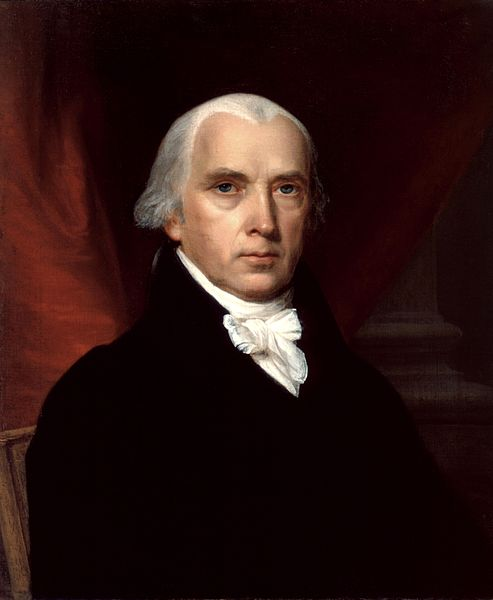
\includegraphics[height=0.4\textheight]{img/madison.jpg} \\
            { \tiny James Madison \\ }
            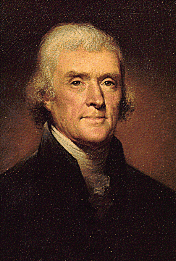
\includegraphics[height=0.4\textheight]{img/jefferson.png} \\
            { \tiny Thomas Jefferson \\ }
    \end{columns}
\end{frame}

\begin{frame}{James Madison, Virginia Resolution, 1798}
    That this Assembly doth explicitly and peremptorily declare, that it views
    the powers of the federal government as resulting from the \textbf{
    \color{blue}compact} to which the states are parties, as limited by
    the plain sense and intention of the instrument constituting that
    \textbf{\color{blue}compact}, as no further valid than they are
    authorized by the grants enumerated in that\textbf{ \color{blue}
    compact}; and that, in case of a deliberate, palpable, and dangerous
    exercise of other powers, not granted by the said\textbf{ \color{blue}
    compact}, the states, who are parties thereto, have the right, and are
    in duty bound, to\textbf{ \color{red}interpose}, for arresting the
    progress of the evil, and for maintaining, within their respective
    limits, the authorities, rights and liberties, appertaining to them.  
\end{frame}

\begin{frame}{Interposition}
    \only<1>{\vspace{10pt}}
    \only<2>{Sovereign states and subdivisions are duty-bound to draw the line}
    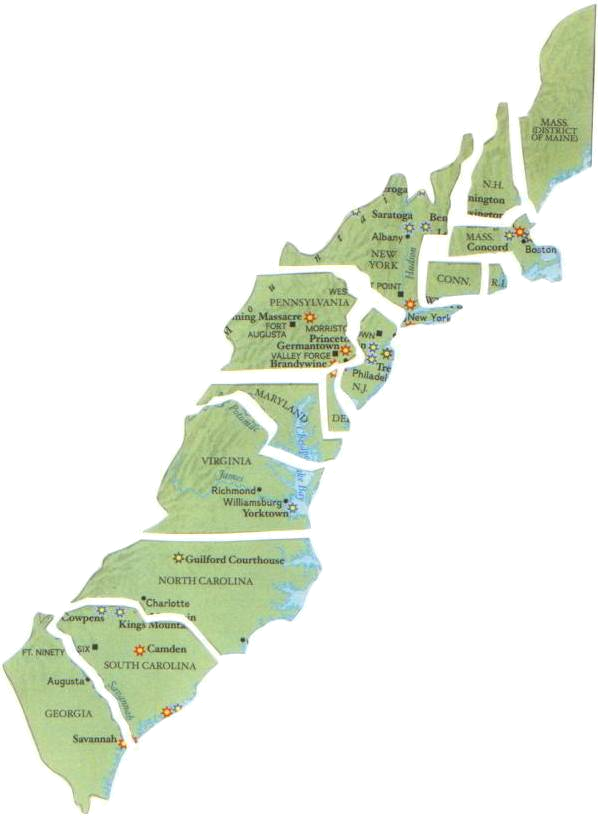
\includegraphics[height=0.75\textheight]{img/colonies.png} \\
    \Put(200,60){
\includegraphics[width=0.3\textwidth]{img/national-seal.png}}
    \Put(100,200){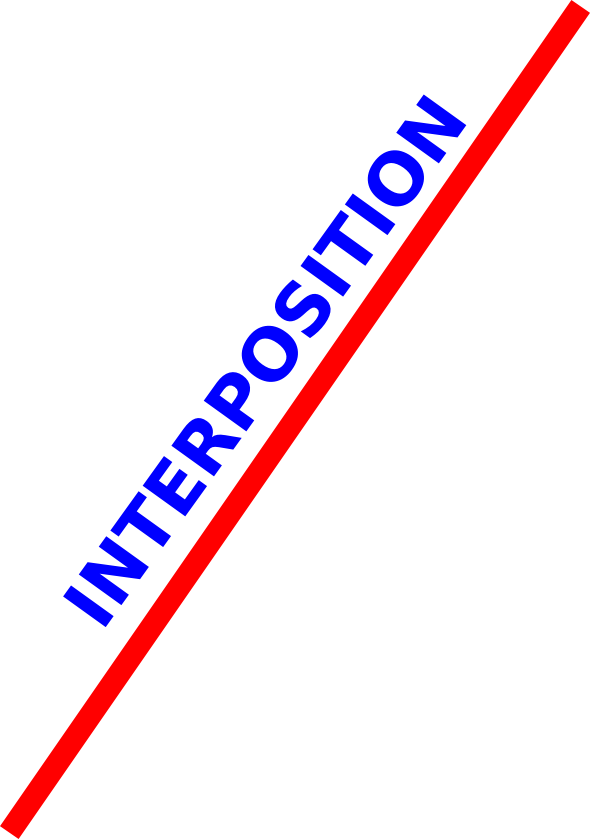
\includegraphics[height=0.8\textheight]{img/line.png}}
\end{frame}

% XXX Do we like this wording? It reappears at the end of section 3
\begin{frame}
    \begin{block}{IMPORTANT!}
        { \huge Interposition is \emph{not} violent. It is \emph{peaceful refusal to allow an agent to exceed its authority}.}
    \end{block}
\end{frame}

\begin{frame}{Utah --- Bound by Oath}
    \begin{columns}[c]
        \column{0.5\textwidth}
            \centering
            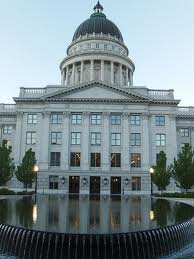
\includegraphics[height=0.9\textheight]{img/utah-capitol.png} \\
        \column{0.5\textheight}
            \centering
            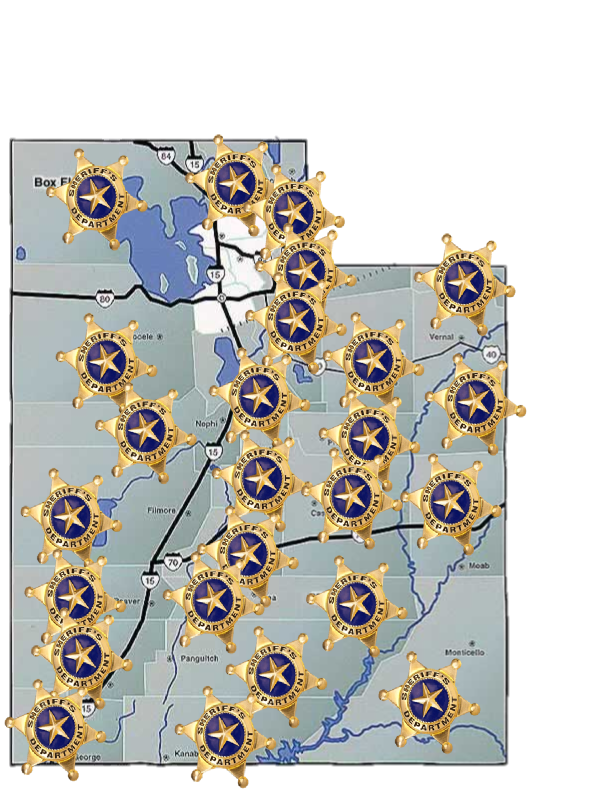
\includegraphics[height=0.9\textheight]{img/utah-sheriffs.png} \\
    \end{columns}
\end{frame}

\begin{frame}
    \begin{columns}[c]
        \column{0.5\textwidth}
            \only<1>{The \textbf{federal} courts have held that the power to declare \textbf{federal} laws unconstitutional lies with the \textbf{federal} courts, not with the states.}
            \only<2>{\centering 
\includegraphics[width=0.8\textwidth]{img/fox-chickens.png} \\}
        \column{0.5\textheight}
            \centering
            
\includegraphics[width=0.9\textwidth]{img/judge-clip.png} \\
    \end{columns}
\end{frame}

\begin{frame}{The Supreme Court}
    \centering
    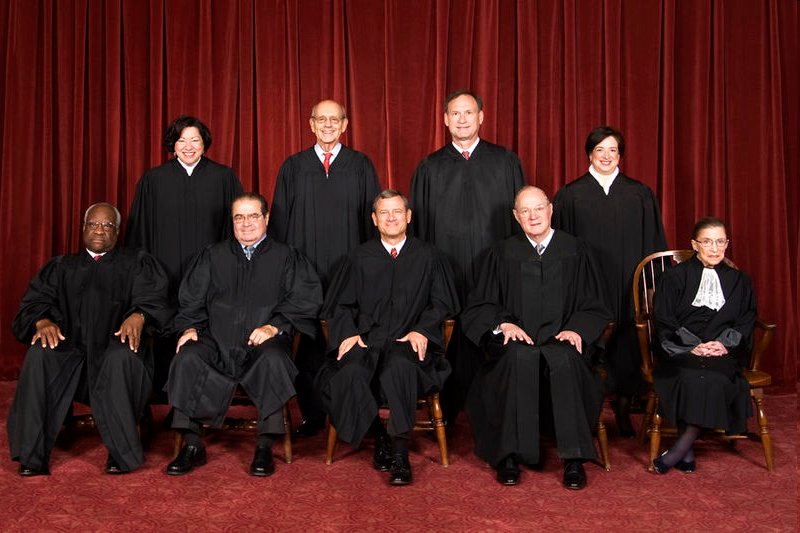
\includegraphics[width=0.9\textwidth]{img/supreme.png} \\
    \only<1>{\large{We are the living Constitution: What we say is what the Constitution means. \\}}
    \only<2>{\large{Interposition is an illegal defiance of Constitutional authority.\\}}
\end{frame}

\begin{frame}{Correction, Please}
    \centering
    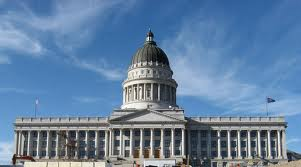
\includegraphics[width=0.9\textwidth]{img/capitol.png} \\
    \large{\emph{\textbf{Interposition}} is a peaceful defiance of illegal unconstitutional authority. \\}
\end{frame}

\begin{frame}
    \centering
    \large{When the legislative, executive, and judicial branches have betrayed us, the states must \textbf{draw the line}, as sentinels of the liberties of the people. \\}
    \includegraphics[height=0.7\textheight]{img/kids.png} \\
\end{frame}

\begin{frame}{Massachussetts, 1809}
    \begin{columns}[c]
        \column{0.5\textwidth}
            \centering
            \includegraphics[width=0.9\textwidth]{img/massachussetts.png} \\
            Massachussetts Legislature, 1809
        \column{0.5\textheight}
            The Embargo Act is ``unconstitutional'' and ``not legally binding on the citizens of this state''. \\
            \vspace{20pt}
            \pause
            \Large{\color{red}Nullification}
    \end{columns}
\end{frame}

\begin{frame}{``Nullification'', 2010}
    \begin{columns}[c]
        \column{0.5\textwidth}
            \centering
            \includegraphics[width=0.9\textwidth]{img/nullification.png} \\
        \column{0.5\textheight}
            \centering
            \only<1>{\includegraphics[width=0.9\textwidth]{img/thomas-woods.png} \\}
            \only<2>{\includegraphics[height=0.4\textheight]{img/ed-phillips.png} \\ Sheriff Ed Phillips \\ Millard County, Utah \\
            \vspace{10pt}
                \large{``I wish to hell that I had had this book in my hands 20 years ago when we started the Western Sheriffs Association.''}
            }
    \end{columns}
\end{frame}

\begin{frame}{Jurisdiction Clause Family --- Guarantee}
    \centering
    \includegraphics[height=0.85\textheight]{img/family.png} \\
    \huge{\textbf{ \color{white}
        %\Put(25, 300){\begin{sideways}\colorbox{blue}{Admissions}\end{sideways}}
        %\Put(60, 300){\begin{sideways}\colorbox{blue}{Claims}\end{sideways}}
        %\Put(90, 300){\begin{sideways}\colorbox{blue}{Property}\end{sideways}}
        \Put(158, 300){\begin{sideways}\colorbox{blue}{Guarantee}\end{sideways}}
        %\Put(168, 300){\begin{sideways}\colorbox{blue}{Enclave}\end{sideways}}
        %\Put(200, 300){\begin{sideways}\colorbox{blue}{Engagements}\end{sideways}}
        %\Put(235, 300){\begin{sideways}\colorbox{blue}{Supremacy}\end{sideways}}
    }}
\end{frame}

\begin{frame}{Guarantee Clause}
    \centering
    \includegraphics[height=.7\textheight]{img/constitution.png} \\
    \textbf{Article IV, Section 4:} ``The United States shall \emph{guarantee} to every State in this Union a \emph{Republican} Form of Government''
\end{frame}

\begin{frame}{Principle of Constitutional Uniformity}
    \centering
    \includegraphics[height=.7\textheight]{img/us-map.png} \\
    \huge{Each state shall be a republic} \\
\end{frame}

\begin{frame}{What kind of republic?}
    \begin{itemize}
        \item Socialist Republic --- government control of all land
        \pause
        \item Aristocratic Republic --- wealthy individuals control government
        \pause
        \item Banana Republic --- deceitful and crafty individuals control government
        \pause
        \item ``the Republic''
    \end{itemize}
\end{frame}

\begin{frame}
    \centering
    \large{``\ldots and to \textbf{the Republic} for which it stands\ldots''} \\
    \includegraphics[width=.9\textwidth]{img/pledge.jpg} \\
\end{frame}

\begin{frame}{The Republic}
    \begin{columns}[c]
        \column{0.5\textwidth}
            \begin{varblock}[0.8\textwidth]{Expert Witness}
                \Large{In the \emph{compound republic} of America\ldots}
            \end{varblock}
        \column{0.5\textheight}
            \centering
            \includegraphics[width=0.9\textwidth]{img/madison.jpg} \\
            James Madison, Father of the Constitution \\
    \end{columns}
\end{frame}

\begin{frame}{The Republic of Republics}
    \begin{columns}[c]
        \column{0.5\textwidth}
            \centering
            \includegraphics[width=0.9\textwidth]{img/republic-of-republics.png} \\
        \column{0.5\textheight}
            \centering
            Bernard Janin Sage \\
            1878, 606 pages \\
    \end{columns}
\end{frame}

\begin{frame}{Who Owns the West?}
    \centering
    \includegraphics[width=.7\textwidth]{img/federal-lands.png} \\
    \pause
    \Large{The Constitutional requirement to \textbf{dispose} of public land was abandoned!} \\
\end{frame}

\begin{frame}
    \begin{block}{In Our Republican Form of Government}
        At the time of statehood, the federal government \emph{relinquished jurisdiction} and proprietary interest over the land with two exceptions:
        \begin{itemize}
            \item Indian lands
            \item Enclaves
        \end{itemize}
    \end{block}
\end{frame}

\begin{frame}{Equal Footing Doctrine}
    \centering
    \includegraphics[width=.7\textwidth]{img/federal-lands.png} \\
    \Large{Admission of new states is ``on an equal footing with the original states in \textbf{all respects whatever}.''} \\
\end{frame}

\begin{frame}{Guarantee Clause has been severely violated}
    \centering
    \includegraphics[height=.7\textheight]{img/constitution.png} \\
    \textbf{Article IV, Section 4:} ``The United States shall \emph{guarantee} to every State in this Union a \emph{Republican} Form of Government''
\end{frame}

\begin{frame}{REMEMBER! Johnson v. McIntosh, 1823}
    \centering
    \includegraphics[width=0.75\textwidth]{img/sc-1905.png} \\
    ``And the \emph{vacant soil is to be disposed of} by that organ of the government which has the constitutional power to dispose of the national domain.'' \\
\end{frame}

\begin{frame}{Law School}
    \centering
    \includegraphics[height=.7\textheight]{img/law-school.png} \\
    \pause
    \large{``Don't read the Constitution. It is too confusing. Here we study case law.''}
\end{frame}

\begin{frame}{United States v. Gratiot, 1840}
    \centering
    \includegraphics[width=0.65\textwidth]{img/sc-1905.png} \\
    \only<1>{
    ``\ldots and this power [over the territorial lands] is vested in Congress
    without limitation, and has been considered the \emph{foundation} upon which the
    \emph{territorial} government rests.''
    }
    \only<2>{
    ``\ldots and this power [over the territorial lands] is vested in Congress
    without limitation {\huge\color{red} \textbf{,}} and has been considered the \emph{foundation} upon which the
    territorial government rests.''
    }
\end{frame}

\begin{frame}{Kleppe v. New Mexico, 1976}
    \centering
    \includegraphics[width=0.65\textwidth]{img/sc-1976.png} \\
    ``We have repeatedly observed that the power over the public lands is thus entrusted to Congress without limitation{ \huge \color{red} \textbf{.}}''
\end{frame}

\begin{frame}{Constitutional Principles of Jurisdiction}
    \begin{columns}[onlytextwidth]
        \column{0.5\textwidth}
            { \large
            Gratiot, 1840: Congress has unlimited power over \textbf{\emph{pre-statehood territorial lands}}. \\
            \vspace{20pt}
            Kleppe, 1976: Congress has unlimited power over \textbf{\emph{``public lands'' within a state}}. \\
            }
        \column{0.5\textwidth}
            \centering
            \includegraphics[width=0.9\textwidth]{img/red-light.png} \\
    \end{columns}
\end{frame}

\begin{frame}{Jurisdiction Clause Family --- Property}
    \centering
    \includegraphics[height=0.85\textheight]{img/family.png} \\
    \huge{\textbf{ \color{white}
        %\Put(25, 300){\begin{sideways}\colorbox{blue}{Admissions}\end{sideways}}
        %\Put(60, 300){\begin{sideways}\colorbox{blue}{Claims}\end{sideways}}
        \Put(105, 300){\begin{sideways}\colorbox{blue}{Property}\end{sideways}}
        %\Put(134, 300){\begin{sideways}\colorbox{blue}{Guarantee}\end{sideways}}
        %\Put(168, 300){\begin{sideways}\colorbox{blue}{Enclave}\end{sideways}}
        %\Put(200, 300){\begin{sideways}\colorbox{blue}{Engagements}\end{sideways}}
        %\Put(235, 300){\begin{sideways}\colorbox{blue}{Supremacy}\end{sideways}}
    }}
\end{frame}

\begin{frame}{August 30, 1787}
    \centering
    \includegraphics[width=0.85\textwidth]{img/convention.png} \\
\end{frame}

\begin{frame}{August 30, 1787}
    \centering
    \includegraphics[width=0.85\textwidth]{img/convention.png} \\
\end{frame}

\begin{frame}{The ``Trust Compacts'' or Engagements, August 30, 1787}
    \begin{columns}[onlytextwidth]
        \column{0.5\textwidth}
            \vspace{10pt}
            \begin{itemize}
                \item The ``Resolution of 1780'' formed the basis upon which Congress was \textbf{required to dispose} of territorial and public lands.
                \item Art. of Confederation, Article IX: ``no State shall be deprived of territory for the benefit of the United States.''
                \item Other state land cession compacts
            \end{itemize}
        \column{0.5\textwidth}
            \centering
            \includegraphics[width=0.85\textwidth]{img/convention.png} \\
    \end{columns}
\end{frame}

\begin{frame}{The ``Trust Compacts'' or Engagements, August 30, 1787}
    \begin{columns}[onlytextwidth]
        \column{0.5\textwidth}
            { \Large It would be best to leave everything on that subject in ``statu quo.'' }
        \column{0.5\textwidth}
            \centering
            \includegraphics[width=0.85\textwidth]{img/convention.png} \\
    \end{columns}
\end{frame}

\begin{frame}{The ``Trust Compacts'' or Engagements, August 30, 1787}
    \begin{columns}[onlytextwidth]
        \column{0.5\textwidth}
            \centering
            \includegraphics[height=0.4\textheight]{img/morris-portrait.png} \\
            { \tiny  Gouvernor Morris } \\
            { \Large ``I make a motion'' \ldots for a property clause} \\
        \column{0.5\textwidth}
            \centering
            \includegraphics[width=0.85\textwidth]{img/convention.png} \\
    \end{columns}
\end{frame}

\begin{frame}{Property Clause}
   \centering
   \includegraphics[height=.7\textheight]{img/constitution.png} \\
   \textbf{Article IV, sec. 3, cl. 2:} ``Congress shall have Power to \emph{dispose of} and make all needful Rules and Regulations respecting the Territory or other \emph{Property} belonging to the United States;''
\end{frame}

\begin{frame}{Property Clause, in \emph{untampered}, plain English}
   \centering
   \includegraphics[height=.7\textheight]{img/constitution.png} \\
   When a territory becomes a state, Congress shall have power to make all needful rules and regulations to \emph{dispose} of former territorial lands and other property in an orderly manner.
\end{frame}

\begin{frame}{Benner v. Porter, 1850}
    \centering
    \includegraphics[width=0.75\textwidth]{img/sc-1905.png} \\
    ``\ldots we are satisfied that \ldots the act of Congress admitting the Territory of Florida, as a State, into the Union \ldots displaced the territorial government, and \emph{abrogated all its powers and jurisdiction.}''
\end{frame}

\begin{frame}{Benner v. Porter, 1850}
    \centering
    \includegraphics[width=0.75\textwidth]{img/sc-1905.png} \\
    ``\ldots the territorial government was displaced, abrogated, every part of it; and that \emph{no power of jurisdiction} existed within her limits, except that derived from State authority.''
\end{frame}

\begin{frame}{Jurisdiction Clause Family --- Enclave}
    \centering
    \includegraphics[height=0.85\textheight]{img/family.png} \\
    \huge{\textbf{ \color{white}
        %\Put(25, 300){\begin{sideways}\colorbox{blue}{Admissions}\end{sideways}}
        %\Put(60, 300){\begin{sideways}\colorbox{blue}{Claims}\end{sideways}}
        %\Put(105, 300){\begin{sideways}\colorbox{blue}{Property}\end{sideways}}
        %\Put(134, 300){\begin{sideways}\colorbox{blue}{Guarantee}\end{sideways}}
        \Put(198, 300){\begin{sideways}\colorbox{blue}{Enclave}\end{sideways}}
        %\Put(200, 300){\begin{sideways}\colorbox{blue}{Engagements}\end{sideways}}
        %\Put(235, 300){\begin{sideways}\colorbox{blue}{Supremacy}\end{sideways}}
    }}
\end{frame}

\begin{frame}{Enclave Clause}
   \centering
   \includegraphics[height=.6\textheight]{img/constitution.png} \\
   \textbf{Article I, sec. 8, cl. 17:} ``Congress shall have power \ldots To
   exercise exclusive Legislation \ldots over all Places \emph{purchased by the
   Consent of the Legislature of the State} in which the Same shall be, for the
   Erection of Forts, Magazines, Arsenals, dock-Yards and other needful
   Buildings.''
\end{frame}

\begin{frame}{Who Owns the West?}
    \centering
    \includegraphics[width=.7\textwidth]{img/federal-lands.png} \\
    \Large{Were the ``western lands'' ``purchased by the Consent of the Legislature of the State''?} \\
\end{frame}

\begin{frame}{Fundamental Principle}
   \centering
   \includegraphics[height=.6\textheight]{img/constitution.png} \\
   \textbf{Fundamental Principle:} By the Constitution only the States can
   create parks, forest reserves, wildlife refuges, monuments, etc. The
   federal government may hold \textbf{no} land in a state for
   non-constitutional purposes.
\end{frame}

\begin{frame}{Federal Attorneys, 2012}
    \begin{columns}[c]
        \column{0.5\textwidth}
            \centering
            Incorrect\ldots \\
            incorrect\ldots \\
            misguided\ldots \\
            Property Clause\ldots \\
            Property Clause\ldots \\
            Property Clause\ldots \\
            Supremacy Clause\ldots \\
            numerous court decisions\ldots \\
            federal laws\ldots \\
            NO STATE CONSENT NECESSARY! \\
        \column{0.5\textwidth}
            \centering
            \includegraphics[height=0.5\textheight]{img/elmer-dickens.png} \\
            Amanda Marshall \\
            Kenneth Paur \\
    \end{columns}
\end{frame}

\begin{frame}{Federal Attorneys, 2012}
\begin{table}[h]
\centering
\begin{tabular}{p{.20\textwidth} p{.70\textwidth}} 
    { \tiny Attorney Dickens } &
        \multirow{2}{.7\textwidth}{ ``There are many US Supreme Court cases going
        back \emph{over a hundred years} where the court has found that Congress has
        broad authority under the Property Clause.''} \\
        { \includegraphics[height=0.15\textheight]{img/elmer-dickens.png} } & \\
    { \tiny Attorney Marshall } & 
        \multirow{2}{.7\textwidth}{``Supreme Court precedent for the \emph{past one hundred years} is clear: under the Property Clause Congress may delegate rule making authority to the federal agencies.'' } \\
        { \includegraphics[height=0.15\textheight]{img/amanda-marshall.png} } & \\
    { \tiny Attorney Paur } & 
        \multirow{2}{.7\textwidth}{``Authority of the Secretary of Agriculture\ldots recognized for \emph{over one hundred years}\ldots Property Clause\ldots Property Clause\ldots'' (20X)} \\
        { \includegraphics[height=0.15\textheight]{img/elmer-dickens.png} } & \\
\end{tabular}
\end{table}
\end{frame}

\begin{frame}{Constitutional Fortress}
    \centering
    \includegraphics[width=0.75\textwidth]{img/fortress.png} \\
    \pause
    \Put(10,180){\includegraphics[width=0.3\textwidth]{img/family.png}}
    \pause
    { \color{red} \huge{Nationalist Assault} \\}
    \pause
    \Put(40,180){\includegraphics[width=0.3\textwidth]{img/property-ram.png}}
    \pause
    \Put(140,180){\includegraphics[width=0.3\textwidth]{img/supremacy-ram.png}}
\end{frame}

\begin{frame}{Constitutional Fortress}
    \centering
    \includegraphics[width=0.75\textwidth]{img/fortress.png} \\
    \Put(10,180){\includegraphics[width=0.3\textwidth]{img/family.png}}
    { \color{red} \huge{Nationalist Assault} \\}
    \Put(90,220){\includegraphics[width=0.3\textwidth]{img/blam.png}}
    \Put(40,180){\includegraphics[width=0.3\textwidth]{img/property-ram.png}}
    \Put(140,180){\includegraphics[width=0.3\textwidth]{img/supremacy-ram.png}}
\end{frame}

\begin{frame}{The Federal Position}
    \begin{columns}[c]
        \column{0.3\textwidth}
            \centering
            \includegraphics[width=0.75\textwidth]{img/elmer-dickens.png} \\
            Attorney Kenneth Paur \\
            Nov. 10, 2011 \\
            Property Clause x 20 \\
        \column{0.7\textwidth}
            The Property Clause provides separate and independent authority for
            Congress to make rules respecting federal property, without
            qualification or limitation. \ldots  Under the Supremacy Clause,
            federal statutes enacted pursuant to the Property clause preempt
            conflicting state laws.
    \end{columns}
\end{frame}

\begin{frame}
    \begin{varblock}[.8\textwidth]{Problem}
        The wellspring of USFS and BLM power is judicial misconstruction of the Property Clause.
    \end{varblock}
\end{frame}

\begin{frame}
    \begin{columns}[c]
        \column{0.5\textwidth}
            \centering
            \includegraphics[height=0.75\textheight]{img/htwwl.png} \\
            2000, 446 pages \\
        \column{0.5\textwidth}
            \centering
            \includegraphics[height=0.35\textheight]{img/william-hayward.png} \\
            { \large The Theft and Usurpation of State's Property Rights }
    \end{columns}
\end{frame}

\begin{frame}
    \begin{columns}[c]
        \column{0.5\textwidth}
            \centering
            \includegraphics[height=0.35\textheight]{img/william-hayward.png} \\
            William Hayward, Page 384 \\
        \column{0.5\textwidth}
            ``In this case [Utah Power \& Light v. United States, 1917], \emph{as in all others I have examined}, [federal land ownership] was not decided; it was \emph{assumed}.''
    \end{columns}
\end{frame}

\begin{frame}
    \begin{columns}[c]
        \column{0.5\textwidth}
            \centering
            \includegraphics[height=0.75\textheight]{img/htwwl.png} \\
            2000 \\
        \column{0.5\textwidth}
            Page 149 \\
            {\Large Eight Supreme Court cases support: \emph{Federal jurisdiction can only occur \textbf{{\color{red} with the consent}} of the legislature of the state. }}
    \end{columns}
\end{frame}

\begin{frame}{Orwellian Doublethink}
    \centering
    \includegraphics[width=.85\textwidth]{img/orwell.png} \\
    \Put(5,85){\includegraphics[width=.3\textwidth]{img/1984.png}}
\end{frame}

\begin{frame}{Orwellian Doublethink}
    \vspace{1pt}
    { \Large
    \textbf{Enclave Clause:} State consent \emph{is} necessary for the Federal Government to build a Post Office within a state \\
    \vspace{20pt}
    \pause
    \textbf{Contemporary Interpretation:} \emph{No} state consent is necessary for the Federal Government to establish a 1.6 million acre national monument within a State. \\
    }
    \pause
    \Put(100,200){\includegraphics[with=.4\textwidth]{img/red-light.png}}
\end{frame}

\begin{frame}
    \begin{varblock}[.9\textwidth]{Fundamental Rule of Constitutional Interpretation}
        An enumerated delegation of limited power will NOT be followed by a general grant of power.
    \end{varblock}
\end{frame}

\begin{frame}{Kohl v. United States, 1875}
    \centering
    \includegraphics[width=0.75\textwidth]{img/sc-1905.png} \\
    { \large ``The consent of a State can never be a condition precedent to [the exercise of federal powers].'' }
\end{frame}

\begin{frame}{Ft. Leavenworth R. Ro. v. Lowe, 1885}
    \centering
    \includegraphics[width=0.75\textwidth]{img/sc-1905.png} \\
    The Kohl decision is ``good law,'' ``a doctrine authoritatively declared.'' Congress may exercise jurisdiction over the places it might acquire \emph{without State consent} provided that those places are ``used as a means to carry out the purposes of the government.''
\end{frame}

\begin{frame}{Jurisdiction Clause Family --- Property}
    \centering
    \includegraphics[height=0.85\textheight]{img/family.png} \\
    \huge{\textbf{ \color{white}
        %\Put(25, 300){\begin{sideways}\colorbox{blue}{Admissions}\end{sideways}}
        %\Put(60, 300){\begin{sideways}\colorbox{blue}{Claims}\end{sideways}}
        \Put(108, 300){\begin{sideways}\colorbox{blue}{Property}\end{sideways}}
        %\Put(134, 300){\begin{sideways}\colorbox{blue}{Guarantee}\end{sideways}}
        %\Put(168, 300){\begin{sideways}\colorbox{blue}{Enclave}\end{sideways}}
        %\Put(200, 300){\begin{sideways}\colorbox{blue}{Engagements}\end{sideways}}
        %\Put(235, 300){\begin{sideways}\colorbox{blue}{Supremacy}\end{sideways}}
    }}
\end{frame}

\begin{frame}{Property Clause}
   \centering
   \includegraphics[height=.7\textheight]{img/constitution.png} \\
   \textbf{Article IV, sec. 3, cl. 2:} ``Congress shall have Power to \emph{dispose of} and make all needful Rules and Regulations respecting the Territory or other \emph{Property} belonging to the United States;''
\end{frame}

\begin{frame}{\st{Property Clause} Disposal Clause}
   \centering
   \includegraphics[height=.7\textheight]{img/constitution.png} \\
   \textbf{Article IV, sec. 3, cl. 2:} ``Congress shall have Power to \emph{dispose of} and make all needful Rules and Regulations respecting the Territory or other \emph{Property} belonging to the United States;''
\end{frame}

\begin{frame}{``Disposal'' Clause, in \emph{untampered}, plain English}
   \centering
   \includegraphics[height=.7\textheight]{img/constitution.png} \\
   \only<1>{When a territory becomes a state, Congress shall have power to make all needful rules and regulations to \emph{dispose} of former territorial lands and other property in an orderly manner. \\ }
   \only<2>{This gives Congress the power to \emph{dispose} of federal lands, not the power \emph{not to dispose} of them. \\}
\end{frame}

\begin{frame}{News Release}
    \begin{block}{March 23, 2012}
    SALT LAKE CITY - Today, Utah Governor Gary R. Herbert signed House Bill
    148, which demands the federal government make good on the promises made in
    the 1894 Enabling Act to extinguish title to federal lands in Utah. 
    \end{block}
\end{frame}

\begin{frame}
    \begin{columns}[c]
        \column{0.5\textwidth}
            \centering
            \includegraphics[width=0.75\textwidth]{img/thomas-paine.png} \\
            Thomas Paine, 1737 - 1809 \\
        \column{0.5\textwidth}
            ``All power exercised over a nation must have some beginning. It
            must either be delegated or assumed. There are no other sources.
            All delegated power is trust, and all assumed power is usurpation.
            Time does not alter the nature and quality of either.''
    \end{columns}
\end{frame}

\begin{frame}
   \centering
   \includegraphics[height=.99\textheight]{img/the-end.png} \\
\end{frame}

\end{document}
